\documentclass{article}
\usepackage[utf8]{inputenc}
\usepackage[T1]{fontenc}
\usepackage[spanish]{babel}
\usepackage[a4paper]{geometry}
%\geometry{top=2.0cm, bottom=2.0cm, left=2.25cm, right=2.25cm}
\usepackage[sorting=none]{biblatex}
\addbibresource{sample.bib}
\usepackage{float}
\usepackage{graphicx}
\usepackage{wrapfig}
\usepackage{subcaption}
\usepackage{amsmath}
\usepackage{amsfonts}
\usepackage{lipsum}  
\usepackage{csquotes}
\usepackage{minted}
\usepackage[hidelinks]{hyperref}

\setlength{\parindent}{0cm}
\renewcommand{\listingscaption}{Código}


\begin{document}

    \begin{titlepage}
    \centering
    {\bfseries\LARGE Universidad Nacional de Ingeniería \par}
    \vspace{1cm}
    {\scshape\Large Facultad de Ciencias \par}
    \vspace{2cm}
    {
\includegraphics[width=0.4\textwidth]{img/uni_logo.png}\par}
    \vspace{2cm}
    {\scshape\Large Estudio Computacional del Problema de los 3 Cuerpos \par}
    \vfill
    {\itshape\Large Seminario de tesis I \par}
    \vfill
    {\Large Autor: \par}
    {\Large Junior Ulises Guevara Tanta \par}
    \vfill
    {\Large Asesor: \par}
    {\scshape\Large Chulluncuy Reynoso  Americo Andres \par}
    \vfill
    {\Large (Lima - Perú) \par}
    {\Large 2023 \par}
    \end{titlepage}

\tableofcontents 


\section{Resumen}
Breve introducción al Problema de los 3 Cuerpos. \newline
Descripción de la motivación para el estudio computacional. \newline
Declaración de los objetivos del proyecto. \newline

\section{Introducción}
El dilema relacionado con los tres cuerpos implica el análisis 
del movimiento de tres objetos que interactúan entre sí de 
acuerdo con las leyes del movimiento de Newton y la ley 
de gravitación universal de Newton. Mientras que el caso 
de dos cuerpos que se influyen gravitacionalmente se 
puede resolver por completo y fue solucionado por 
Newton en el siglo XVII , el caso de tres cuerpos
no se resolvió por completo y se convirtió en un 
problema de gran relevancia en el siglo XVIII \cite{musielak2014three}. En 
tiempos recientes, el problema de los tres cuerpos ha 
adquirido una considerable importancia debido a sus numerosas 
aplicaciones en Astronomía, como por ejemplo en la investigación 
de exoplanetas y en la determinación de las trayectorias 
de naves espaciales. //


En el siglo XVIII, Euler y Lagrange lograron encontrar 
soluciones analíticas para este problema bajo un conjunto 
específico de condiciones iniciales, es decir, las 
posiciones iniciales y velocidades de los cuerpos. 
Estas dos soluciones son las únicas soluciones explícitas 
conocidas para el problema completo de los tres cuerpos. 
Durante este período, Euler también se ocupó del sistema 
Sol-Tierra-Luna, considerando que la Luna carece de masa, 
lo que hoy se conoce como el problema restringido de 
los tres cuerpos. Sin embargo, fue necesario esperar 
hasta el siglo XX para obtener una solución en forma 
de serie para el problema de los tres cuerpos, la cual 
es aplicable en la mayoría de las condiciones iniciales, 
especialmente cuando el momento angular total del sistema 
no es igual a cero. No obstante, estas soluciones en 
serie resultan prácticamente inutilizables en la práctica 
debido a su convergencia extremadamente lenta, lo que 
impide extraer información útil de ellas. Por lo tanto, 
es imprescindible recurrir a métodos numéricos para 
obtener soluciones al problema de los tres cuerpos \cite{musielak2014three}.\\


En los últimos años, se han descubierto varias 
soluciones al enigma de los tres cuerpos, 
aunque la mayoría de ellas se caracterizan 
por su falta de estabilidad. Sin embargo, 
para abordar este análisis de manera efectiva, 
resulta fundamental definir el método a utilizar. 
Con este propósito, se realizará una 
evaluación exhaustiva de diferentes métodos y se 
llevará a cabo una comparación entre ellos. \\

 
\section{Formulación matemática}
Los desplazamientos de tres objetos que experimentan 
interacciones gravitacionales se rigen por las leyes 
del movimiento de Newton y la ley de gravitación 
universal de Newton. En el caso de cuerpos con 
masas $m_1$, $m_2$ y $m_3$, ubicados en 
posiciones $r_1$, $r_2$ y $r_3$, se pueden 
expresar las ecuaciones de movimiento de la 
siguiente manera \cite{montgomery2001new}: \\


\begin{equation}
    \begin{split}
    \Ddot{r_1} = -G \frac{m_2(r_1 - r_2 )}{{| r_1 - r_2 |}^3} - G \frac{m_3(r_1 - r_3)}{{| r_1 - r_3 |}^3}  \\
    \Ddot{r_2} = -G \frac{m_1(r_2 - r_1 )}{{| r_2 - r_1 |}^3} - G \frac{m_3(r_2 - r_3)}{{| r_2 - r_3 |}^3} \\
    \Ddot{r_3} = -G \frac{m_1(r_3 - r_1 )}{{| r_3 - r_1 |}^3} - G \frac{m_2(r_3 - r_2)}{{| r_3 - r_2 |}^3}
    \end{split}
\end{equation}


Cuando nos enfocamos en un movimiento limitado a un plano, nos 
encontramos con un sistema de seis ecuaciones diferenciales 
ordinarias (EDO) de segundo orden. Sin embargo, es comúnmente 
ineficiente tratar con EDOs de segundo orden, y resulta 
mucho más práctico abordar EDOs de primer orden. 
Si consideramos las posiciones $r_i$ de los cuerpos y sus velocidades $v_i$ 
de manera separada, podemos reformular este sistema como un 
conjunto de EDOs de primer orden: \\


\begin{equation}
    \begin{split}
    \dot{r_1} &= v_1 \\
    \dot{r_2} &= v_2 \\
    \dot{r_3} &= v_3 \\
    \dot{v_1} &= -G \frac{m_2(r_1 - r_2 )}{{| r_1 - r_2 |}^3} - G \frac{m_3(r_1 - r_3)}{{| r_1 - r_3 |}^3}  \\
    \dot{v_2} &= -G \frac{m_1(r_2 - r_1 )}{{| r_2 - r_1 |}^3} - G \frac{m_3(r_2 - r_3)}{{| r_2 - r_3 |}^3} \\
    \dot{v_3} &= -G \frac{m_1(r_3 - r_1 )}{{| r_3 - r_1 |}^3} - G \frac{m_2(r_3 - r_2)}{{| r_3 - r_2 |}^3}
    \end{split}
\end{equation}


Cuando se trata de un movimiento restringido al plano, 
nos enfrentamos a un conjunto de 12 ecuaciones 
diferenciales ordinarias de primer orden. 
En este tipo de sistema, existen ciertas 
cantidades conocidas como integrales de movimiento 
que se mantienen constantes, incluyendo la 
energía total $E$ del sistema, el momento 
angular total $L$ del sistema (es importante 
destacar que este es un vector y, además, es 
perpendicular al plano del movimiento, es decir, el plano $xy$), 
y el momento lineal del centro de masa, $P$. 
En consecuencia, al obtener cualquier solución 
numérica para el problema de los tres cuerpos, 
estas magnitudes se conservan \cite{musielak2014three}. Podemos expresar estas 
cantidades de manera explícita como se indica a continuación : \\

\begin{align}
    E &= \frac{1}{2} \sum_{i=1}^3 m_i {|v_i|}^2 - G\sum_{\substack{i=1 \\ j < i}}^3 \frac{m_im_j}{|r_i - r_j|} \\
    L &= \left| \sum_{i = 1}^3 m_ir_i \times v_i \right| \\
    P &= \sum_{i=1}^3m_iv_i
\end{align}


\section{ Soluciones conocidas del problema de los tres cuerpos}

\subsection{Orbitas clasicas}
Como se explicó en la introducción, aunque el sistema que 
describe el movimiento de tres cuerpos que interactúan 
gravitatoriamente no puede, en términos generales, 
resolverse de manera analítica, se han identificado 
dos soluciones analíticas específicas, atribuidas a 
Euler y Lagrange. En la órbita de Euler, los tres 
cuerpos inician en una disposición lineal, y los 
dos cuerpos exteriores siguen una trayectoria 
circular alrededor del cuerpo central, que se ubica 
en el centro de este círculo (consulte la Figura 1a). 
En la órbita de Lagrange, los tres cuerpos parten 
desde los vértices de un triángulo equilátero y 
siguen una trayectoria circular, manteniendo la 
estructura triangular en todo momento (ver Figura 1b) 
\cite{montgomery2001new}.


\begin{figure}[h]

\begin{subfigure}{0.5\textwidth}
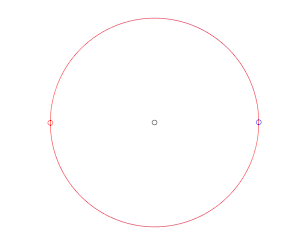
\includegraphics[width=0.9\linewidth, height=6cm]{img/EulerOrbit.png} 
\caption{Órbita de Euler}
\label{fig:subim1}
\end{subfigure} 
\begin{subfigure}{0.5\textwidth}
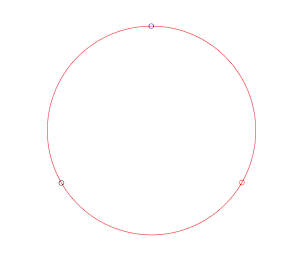
\includegraphics[width=0.9\linewidth, height=6cm]{img/LagrangeOrbit.png}
\caption{Órbita de Lagrange}
\label{fig:orbit1}
\end{subfigure}

\caption{Órbitas clásicas de tres cuerpos}
\label{fig:image2}
\end{figure}


A pesar de que estas soluciones se describen con expresiones 
analíticas precisas, presentan inestabilidad, lo 
que significa que pequeñas variaciones en las 
condiciones iniciales resultan en cambios 
significativos en el comportamiento de largo 
plazo de los cuerpos. En términos generales, 
encontrar órbitas que no sean inestables resulta 
una tarea desafiante. Sin embargo, existe una 
órbita estable conocida para sistemas con $N > 2$ 
y tres masas iguales, y se trata de la 
órbita de tres cuerpos en forma de 8 \cite{montgomery2001new}.

\subsection{Órbita de la Figura 8}
La órbita en forma de figura 8, también conocida como la órbita 
de la figura-8, representa la única solución estable que se 
conoce hasta ahora para el problema de los tres cuerpos. 
En esta órbita particular, los tres cuerpos inicialmente 
se alinean en una configuración lineal y luego siguen 
una trayectoria que se asemeja a un número 8, tal 
como se ilustra en la Figura 2 \cite{montgomery2001new}.

\begin{figure}[h]
\centering
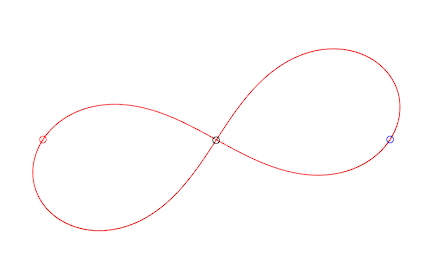
\includegraphics[width=0.5\textwidth]{img/orbit8.png}
\caption{Órbita de la Figura 8}
\end{figure}


Para crear estar orbita la condiciones iniciales son la siguientes \cite{atkinson2011numerical}: 

$$r_1(0) = -r_3(0) = (-0.97000436,0.24208753)$$
$$r_2(0) = (0,0)$$
$$v_1(0) = v_3(0) = (0.4662036850, 0.4323657300)$$
$$v_2(0) = (-0.933240737, -0.86473146)$$
$$m_1 = m_2 = m_3$$


Estas son las posiciones iniciales , $r_1(0)$ y $-r_3(0)$, de las 
partículas 1 y 3, que son idénticas debido a que se 
encuentran en lados opuestos del origen de coordenadas. 
Estas posiciones se representan en un sistema de coordenadas 
bidimensional y se utilizan para definir la disposición 
inicial de dos de las partículas en el sistema. La 
partícula 1 tiene una coordenada x negativa y una 
coordenada y positiva, mientras que la partícula 3 
tiene una coordenada x positiva y una coordenada y 
positiva y $r_2(0)$ esta es la posición inicial de la partícula 2, 
que se encuentra en el origen del sistema de coordenadas.

Las velocidades iniciales, $v_1(0)$ y $v_3(0)$, de las partículas 
1 y 3, que son idénticas debido a que tienen la misma magnitud y 
dirección. Estas velocidades se utilizan para describir 
cómo se están moviendo las partículas 1 y 3 en el momento 
inicial. Ambas partículas tienen componentes en las direcciones 
$x$ e $y$ y $v_2(0)$ esta es la velocidad inicial de la partícula 2, 
que tiene componentes distintas en las direcciones x e y.

Las masas de las tres partículas, denotadas como $m_1$, $m_2$ y $m_3$, 
son iguales. Esto implica que las partículas tienen la misma 
cantidad de masa y, por lo tanto, influyen de manera 
equivalente en las fuerzas gravitatorias que se ejercen entre ellas.

%\subsection{Otras orbitas}


\section{Métodos de integración}
Para resolver el conjunto de ecuaciones diferenciales 
ordinarias (EDO) que describe el movimiento de 
los cuerpos, es necesario recurrir a un solucionador 
numérico para obtener una aproximación de la solución. 
Existen diversos solucionadores disponibles, cada 
uno con diferentes niveles de precisión (orden) y 
propiedades específicas. En este proyecto, se han 
implementado cuatro métodos distintos: 
% Esto puede varias , se pueden agregar mas metodos
Euler, Runge-Kutta de cuarto orden, Verlet y Leapfrog.

Dado que la órbita se desarrolla en un plano, el 
momento angular que se ha considerado en las 
leyes de conservación es la componente $z$, $L_z$. 
Además, los intervalos de tiempo utilizados 
se expresan en relación al período de la órbita, 
que en este caso es igual a 6.325 [3].

\subsection{Metodo de Euler}
Este método es el solucionador numérico de ecuaciones 
diferenciales ordinarias (EDO) más básico. Cuando 
trabajamos con un sistema expresado en forma 
vectorial, como $\dot{y} = f(t, y)$, y un intervalo 
de tiempo $\delta t$, el valor de $y$ en el momento $ t + \delta t$, 
denotado como $y_{i+1}$, se determina en función del 
valor de $y$ en el instante $t$, que es $y_i$. 
Esto se calcula de la siguiente manera \cite{atkinson2011numerical}:

\begin{equation}
    y_{i+1} = y_i + f(t, y_i) \delta t
\end{equation}

Este es un método de primer orden, lo que significa 
que el error en la estimación realizada es proporcional 
al valor del intervalo $\delta t$. Esto implica que el método 
resulta en aproximaciones poco precisas, y se requiere 
seleccionar un paso de tiempo extremadamente reducido 
para lograr una aproximación de calidad \cite{atkinson2011numerical}. 
Esta limitación se refleja en la Figura 4, donde 
se emplearon 1000 intervalos de tiempo por 
período de la órbita.


\begin{figure}[h]
\centering
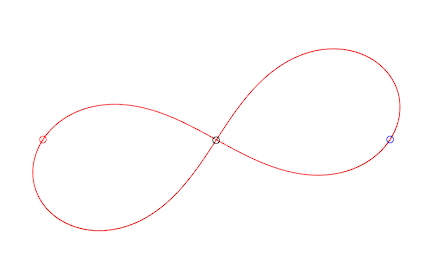
\includegraphics[width=0.5\textwidth]{img/orbit8.png}
\caption{Órbita de la Figura 8 con el método de Euler}
\end{figure}




\printbibliography

\end{document}